\shortappendixtrue

\section{Appendix}

% Data and demand

\gdef\shortbuttons{\hyperlink{short-21}{\beamergotobutton{Back}}}
\begin{frame}[label=short-22,noframenumbering]{Sample Statistics: Purchase Activity}
  \centering
  \small
  \renewcommand{\arraystretch}{1.15}
  \begin{tabular}{lrr}
    \toprule
     & Full sample & Yogurt sample \\
    \midrule
    Households & 37,827 & 15,106 \\
    Observed panel years & 3.96 & 3.16 \\
    Trips per household & 493.13 & 20.26 \\
    Trips per observed week (approx.) & 2.27 & 0.11 \\
    Distinct UPCs per household & 1,178.31 & 13.89 \\
    Purchase lines per household & 3,397.64 & 45.15 \\
    Packages per household & 4,669.07 & 93.77 \\
    \bottomrule
  \end{tabular}

  \medskip
  {\footnotesize All statistics except household counts are means.}
\end{frame}



\gdef\shortbuttons{\hyperlink{short-4}{\beamergotobutton{Back}}}
\begin{frame}[label=short-5,noframenumbering]{Flavor Popularity}
  \centering
    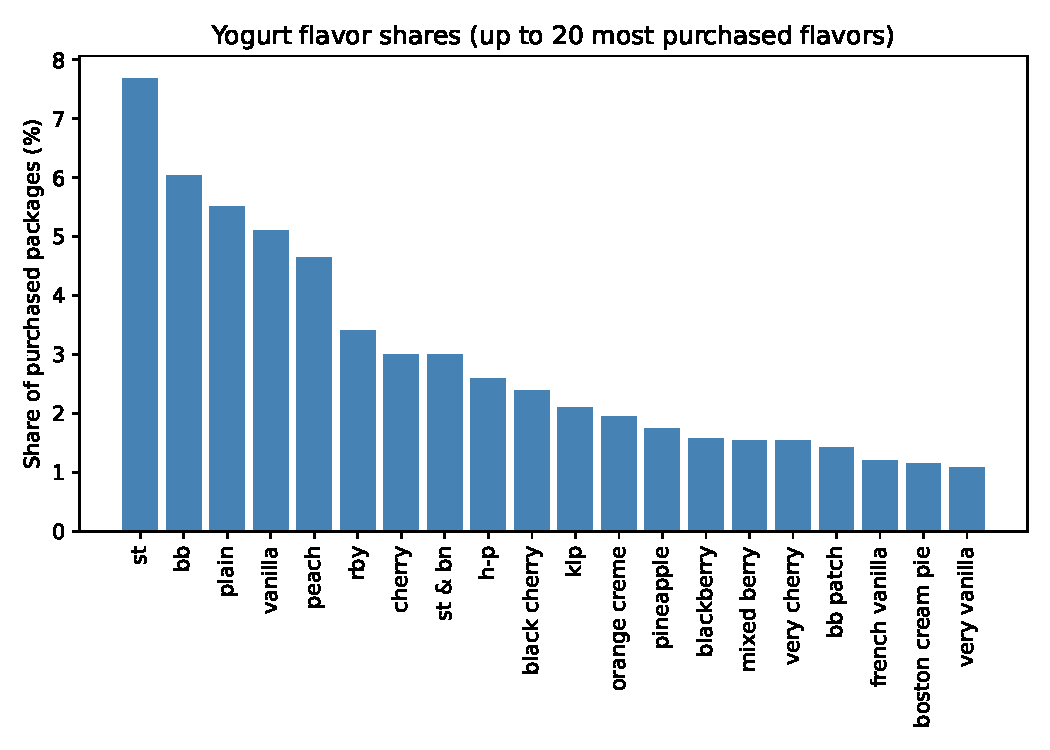
\includegraphics[width=.95\textwidth,height=.74\textheight,keepaspectratio]{../writeup/1108_writeup/assets/results/summary_statistics/flavor_shares.pdf}
\end{frame}



\gdef\shortbuttons{\hyperlink{short-29}{\beamergotobutton{Back to Estimation}}}
\begin{frame}[label=short-demand-fit,noframenumbering]{New Demand Fit: Three Flavors, Average History}
  \centering\small
  \begin{tabular}{lr}\toprule
Specification & Three flavors; no price controls\\
Habit history & Average prior flavor shares\\
Households & 15,105 \\
Household-week observations & 281,695 \\
Negative log likelihood & 1,590,033.03 \\
AIC & 3,180,084.06 \\
BIC & 3,180,152.67 \\
Optimizer & Converged\\\bottomrule\end{tabular}

  \par\medskip\footnotesize November 11 uncontrolled fit; outside count $\max(7-Q,0)$ within retained purchase weeks.
  Novelty uses the preceding calendar week's flavor shares; zero when no yogurt was purchased.
\end{frame}

\gdef\shortbuttons{\hyperlink{short-32}{\beamergotobutton{Back to Distributions}}}
\begin{frame}[label=short-30,noframenumbering]{Demand Estimates and Uncertainty}
  \centering\small
  \begin{adjustbox}{max width=\linewidth}
    \begin{tabular}{lrrr}\toprule
Parameter & Estimate & SE & 95\% interval\\\midrule
Inside constant $\beta_0$ & 0.693 & 0.005 & [0.683, 0.703] \\
Berry vs. other & -0.290 & 0.004 & [-0.298, -0.282] \\
Plain vs. other & 0.006 & 0.006 & [-0.006, 0.018] \\
Mean log price magnitude $\mu_{\log a}$ & -0.536 & 0.006 & [-0.548, -0.524] \\
Mean novelty $\mu_\gamma$ & -0.358 & 0.013 & [-0.383, -0.332] \\
Mean habit $\mu_\phi$ & 0.738 & 0.010 & [0.719, 0.757] \\
SD log price magnitude $\sigma_{\log a}$ & 0.795 & 0.005 & [0.785, 0.805] \\
SD novelty $\sigma_\gamma$ & 1.131 & 0.013 & [1.106, 1.156] \\
SD habit $\sigma_\phi$ & 1.516 & 0.010 & [1.496, 1.536] \\
\bottomrule\end{tabular}

  \end{adjustbox}
  \par\medskip\footnotesize Standard errors from the observed-information Hessian; normal 95\% intervals.
  Standard deviations describe population heterogeneity, not estimation uncertainty.
\end{frame}

\gdef\shortbuttons{\hyperlink{short-32}{\beamergotobutton{Back to Distributions}}}
\begin{frame}[label=short-33,noframenumbering]{What the New Demand Estimates Say}
  \centering
  \begin{tabular}{lrrr}\toprule
Preference & Mean & Population SD & Share positive\\\midrule
Novelty & -0.358 & 1.131 & 37.6\%\\
Habit & 0.738 & 1.516 & 68.7\%\\\bottomrule\end{tabular}

  \begin{itemize}
    \item Most consumers dislike switching; a substantial minority prefer novelty.
    \item Habit preference is positive on average, with wide variation across consumers.
    \item Berry has a negative flavor intercept relative to other. Plain's interval includes zero.
  \end{itemize}
  \par\smallskip\footnotesize Shares are implied by fitted population normal distributions, not counts of classified households.
\end{frame}

\gdef\shortbuttons{\hyperlink{short-29}{\beamergotobutton{Back to Estimation}}}
\begin{frame}[label=short-price-distribution,noframenumbering]{Price Sensitivity: From Log Parameters to Dollar Prices}
  \[
    \alpha_i=-\exp(\mu_{\log a}+\sigma_{\log a}\nu_{\alpha i}),\qquad \nu_{\alpha i}\sim\mathcal N(0,1).
  \]
  \[
    E[\alpha_i]=-\exp(\mu_{\log a}+\tfrac12\sigma_{\log a}^2).
  \]
  \begin{tcolorbox}
    Population mean price coefficient: $E[\alpha_i]=-0.803$.\\
Population standard deviation: $\mathrm{SD}(\alpha_i)=0.753$.

  \end{tcolorbox}
  \begin{itemize}
    \item All consumers have a negative price coefficient.
    \item The quantified theory uses the population mean coefficient in both pricing regimes.
  \end{itemize}
\end{frame}

\gdef\shortbuttons{\hyperlink{short-31}{\beamergotobutton{Back to WTP}}}
\begin{frame}[label=short-wtp-interpretation,noframenumbering]{Interpreting Willingness to Pay}
  \[
    \mathrm{WTP}_{\gamma,i}=\frac{\gamma_i}{-\alpha_i},\qquad
    \mathrm{WTP}_{\phi,i}=\frac{\phi_i}{-\alpha_i}.
  \]
  \begin{itemize}
    \item Novelty: mean WTP is $-\$0.84$ per unit of the novelty predictor.
    \item Habit: mean WTP is $\$1.73$ for a unit increase in the prior average flavor share.
    \item A 10-percentage-point increase in average share corresponds to $\$0.17$ at the mean WTP.
  \end{itemize}
  \begin{tcolorbox}
    Average individual WTP ratios. They need not equal a ratio of mean coefficients.
  \end{tcolorbox}
\end{frame}


\gdef\shortbuttons{\hyperlink{short-27}{\beamergotobutton{Back}}}
\begin{frame}[label=short-average-history,noframenumbering]{Average History: Fitted Specification}
  \[
    H^{\mathrm{avg}}_{ijt}=\frac{1}{n_{it}}
      \sum_{s\in\mathcal{O}_i,\,s<t}w_{ijs},
    \qquad n_{it}=\#\{s\in\mathcal{O}_i:s<t\}.
  \]
  \begin{itemize}
    \item $\mathcal{O}_i$: observed yogurt-purchase weeks; $n_{it}$ counts prior occasions.
    \item Empty history gives zero. Unobserved calendar weeks do not enter the denominator.
    \item Current purchases affect the next state only.
  \end{itemize}
  \begin{tcolorbox}
    Displayed demand estimates use the November 11 three-flavor average-history fit.
    The pricing illustration holds habit at its reference level.
  \end{tcolorbox}
\end{frame}



\gdef\shortbuttons{\hyperlink{short-29}{\beamergotobutton{Back}}}
\begin{frame}[label=short-28,noframenumbering]{Demand Probabilities and the Household Likelihood}
  \[
    P_{ijt}(\nu_i)=\frac{\exp(V_{ijt}(\nu_i))}{1+\sum_k\exp(V_{ikt}(\nu_i))},\qquad
    P_{i0t}(\nu_i)=\frac{1}{1+\sum_k\exp(V_{ikt}(\nu_i))}.
  \]
  \[
    L_i(\theta)=\int\prod_t P(y_{it}\mid\nu_i,\theta)\,f_{\mathcal N}(\nu_i)\,d\nu_i.
  \]
  \begin{itemize}
    \item Within a household-week, observed counts follow the multinomial choice probabilities.
    \item Integrate the product over time: household tastes persist across observed weeks.
    \item Taste heterogeneity and transitory logit shocks play different roles.
  \end{itemize}
\end{frame}



% Theory details

\gdef\shortbuttons{\hyperlink{short-14}{\beamergotobutton{Back}}}
\begin{frame}[label=short-12,noframenumbering]{Pricing Simulations Specification}
  \centering
  \small
  \begin{tabular}{lll}
    \toprule
    Parameter & Description & Value \\
    \midrule
    $\beta$ & Inside-good intercept & $2$ \\
    $\alpha$ & Price sensitivity & $1$ \\
    $\delta$ & Discount factor (no discounting) & $1$ \\
    $c$ & Marginal cost & $0$ \\
    $\gamma$ & Switching preference & $[-3,3]$ \\
    \midrule
    \multicolumn{2}{l}{Initial Consumption State}
      & $h_0\in\{0,j\}$ \\
    \multicolumn{2}{l}{Feasible Prices}
      & $p_t(h)\in\mathbb{R}$ \\
    \bottomrule
  \end{tabular}
  \begin{itemize}
    \item Allow for negative pricing
    \item Firm has knowledge of both type and history, allowing for targeted pricing
    \item Four consumption histories possible $(h_0, h_1) \in \{(0,0), (0,j), (j,j), (j,0)\}$
  \end{itemize}
\end{frame}



\gdef\shortbuttons{\hyperlink{short-10}{\beamergotobutton{Back}}}
\begin{frame}[label=short-52,noframenumbering]{Shares and Elasticities}
  \begin{tcolorbox}
    [
    boxsep=0pt,
    left=2pt, right=2pt,
    top=1pt, bottom=1pt,
    before skip=2pt, after skip=2pt
    ]
    \setlength{\abovedisplayskip}{2pt}
    \setlength{\belowdisplayskip}{2pt}
    \begin{gather*}
      s_t(h) = \frac{e^{v_t(h)}}{1+e^{v_t(h)}}, \ s_{0t}(h) = 1-s_t(h) \\
      \frac{\partial s_t(h)}{\partial p_t(h)} = -\alpha s_t(h)(1-s_t(h)) \\
      \frac{\partial s_t(h)}{\partial\gamma} = q(h)s_t(h)(1-s_t(h))
    \end{gather*}
  \end{tcolorbox}
  \end{frame}



\gdef\shortbuttons{\hyperlink{short-10}{\beamergotobutton{Back}}}
\begin{frame}[label=short-9,noframenumbering]{Optimal Terminal Price and Profit}
  \begin{tcolorbox}
    [
    boxsep=0pt,
    left=2pt, right=2pt,
    top=1pt, bottom=1pt,
    before skip=2pt, after skip=2pt
    ]
    \setlength{\abovedisplayskip}{2pt}
    \setlength{\belowdisplayskip}{2pt}
    \begin{align*}
      \frac{\partial\pi_2(h_1)}{\partial p_2(h_1)} &= s_2(h_1) + (p_2 - c)\frac{\partial s_2(h_1)}{\partial p_2(h_1)} \\
      p_2^*(h_1)&= c + \frac{1}{\alpha(1-s_2^*(h_1))} \\
      \pi^*_2(p_2^*(h_1); h_1) &= \frac{s_2^*(h_1)}{\alpha(1-s_2^*(h_1))}
    \end{align*}
  \end{tcolorbox}
  \begin{itemize}
    \item Optimal period two price is cost plus a demand markup term
    \item Period two profit at optimal prices is the odds of purchase, scaled by the inverse price sensitivity
  \end{itemize}
\end{frame}



\gdef\shortbuttons{\hyperlink{short-10}{\beamergotobutton{Back}}}
\begin{frame}[label=short-11,noframenumbering]{Optimal Profit Given Switching Type}
  \begin{tcolorbox}
    [
    boxsep=0pt,
    left=2pt, right=2pt,
    top=1pt, bottom=1pt,
    before skip=2pt, after skip=2pt
    ]
    \setlength{\abovedisplayskip}{2pt}
    \setlength{\belowdisplayskip}{2pt}
    \begin{align*}
      \frac{d\Pi}{d\gamma} &= \frac{q(h)s_1^*(h) - \delta s_1^*(h)s_2^*(j) + \delta(1-s_1^*(h))s_2^*(0)}{\alpha}
    \end{align*}
  \end{tcolorbox}
  \begin{itemize}
    \item Initially outside: optimal profit increases with the switching preference.
    \item Initially inside: switching changes both retention and the value of a future return; the net effect can change sign.
  \end{itemize}
\end{frame}



\gdef\shortbuttons{\hyperlink{short-14}{\beamergotobutton{Back}}}
\begin{frame}[label=short-13,noframenumbering]{Theory: Numerical Price and Profit Benchmarks}
  \begin{center}\small\begin{tabular}{crrrrrr}\toprule
  $x_0$ & $\gamma$ & $p_1^*$ & $p_2^*(j)$ & $p_2^*(0)$ & $\Pi^*$ & $\Pi^{*\prime}$\\\midrule
  $j$ & -3 & 3.358 & 3.926 & 1.120 & 5.284 & -1.445\\
  $j$ & -1 & 2.211 & 2.557 & 1.567 & 2.768 & -0.993\\
  $j$ & 0 & 2.000 & 2.000 & 2.000 & 2.000 & -0.500\\
  $j$ & 1 & 2.271 & 1.567 & 2.557 & 1.838 & 0.177\\
  $j$ & 3 & 3.814 & 1.120 & 3.926 & 2.934 & 0.730\\
  $0$ & -3 & -0.901 & 3.926 & 1.120 & 1.026 & 0.177\\
  $0$ & -1 & 1.005 & 2.557 & 1.567 & 1.562 & 0.376\\
  $0$ & 0 & 2.000 & 2.000 & 2.000 & 2.000 & 0.500\\
  $0$ & 1 & 2.995 & 1.567 & 2.557 & 2.562 & 0.624\\
  $0$ & 3 & 4.905 & 1.120 & 3.926 & 4.025 & 0.823\\
  \bottomrule\end{tabular}\end{center}
\end{frame}



\gdef\shortbuttons{\hyperlink{short-20}{\beamergotobutton{Back}}}
\begin{frame}[label=short-54,noframenumbering]{Fixed Beliefs for Offers; Persistent Types for Evaluation}
  \begin{itemize}
    \item The hidden-type firm uses $\mu_r$ in every state to choose offers;
    it does not update beliefs after a purchase.
    \item Real consumers retain their type. First-period choices sort types into
    histories even when the firm ignores that information.
  \end{itemize}
  \[
    \Pr(j\text{ in both periods})=\sum_r\mu_r s_{1r}s_{2r}(j),
    \quad\text{not}\quad
    \left(\sum_r\mu_r s_{1r}\right)\left(\sum_r\mu_r s_{2r}(j)\right).
  \]
  \begin{tcolorbox}
    The firm's fixed-belief optimization objective and realized persistent-type
    revenue need not coincide. All displayed policy comparisons use the latter.
  \end{tcolorbox}
\end{frame}



\gdef\shortbuttons{\hyperlink{short-20}{\beamergotobutton{Back to Theory Comparison}}}
\begin{frame}[label=short-19,noframenumbering]{Theory: Revenue Levels under the Same Persistent Types}
  \centering
  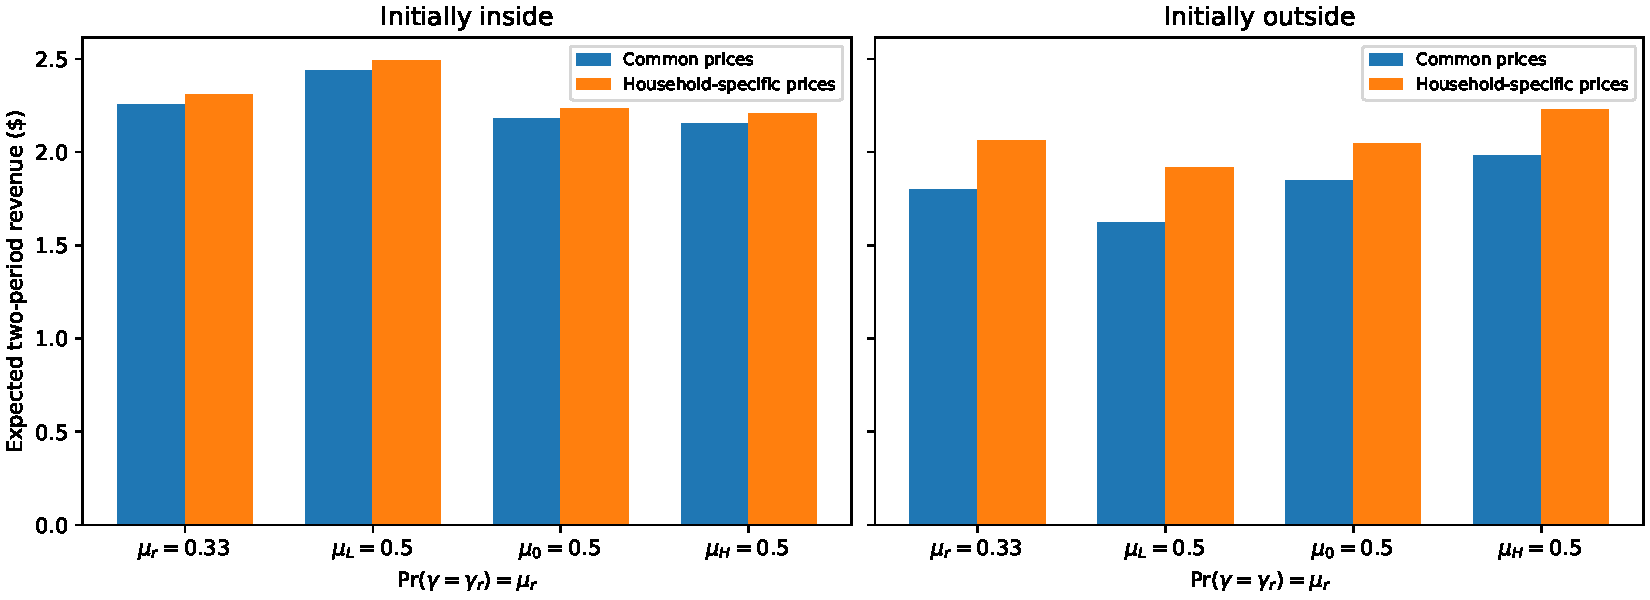
\includegraphics[width=.98\textwidth,height=.72\textheight,keepaspectratio]{assets/theory_delta1/gamma_uncertainty/profits.pdf}
  \par\smallskip\footnotesize Full-information optimal revenue versus realized revenue of the fixed-belief common policy.
\end{frame}

\gdef\shortbuttons{\hyperlink{short-20}{\beamergotobutton{Back to Theory Comparison}}}
\begin{frame}[label=short-53,noframenumbering]{Theory: Type-Specific and Common Offers}
  \centering
  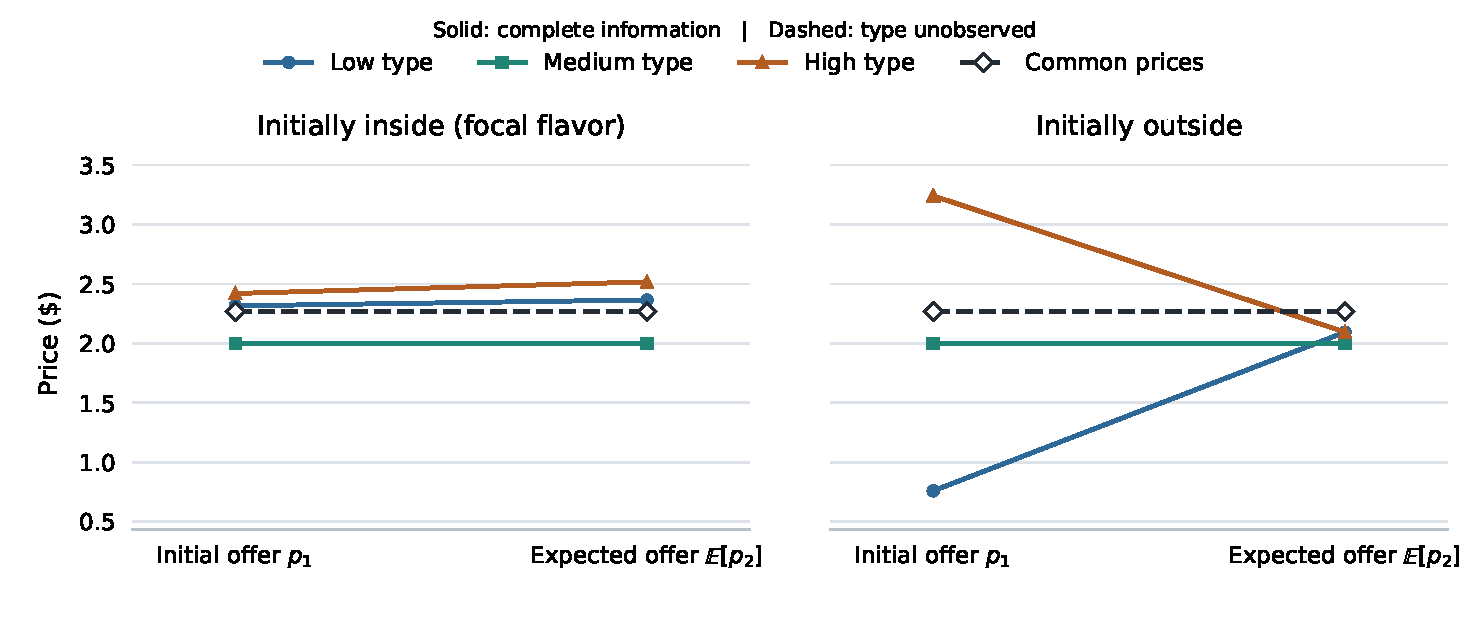
\includegraphics[width=.98\textwidth,height=.70\textheight,keepaspectratio]{assets/theory_delta1/gamma_uncertainty/information_price_paths_comparison.pdf}
  \par\smallskip\footnotesize Equal type weights; same format as the quantified plain price paths.
\end{frame}

% Quantified theory details

\gdef\shortbuttons{\hyperlink{short-34}{\beamergotobutton{Back to Quantified Theory}}}
\begin{frame}[label=short-theory-mapping,noframenumbering]{Exactly What Maps from Demand to Theory?}
  \[
    v_t=\beta_f-a p_t+\gamma q(h_t),\qquad a=-E[\alpha_i]=0.803.
  \]
  \centering
  \begin{tabular}{lr}\toprule
    Input & November 11 estimate\\\midrule
    Plain intercept $\beta_0+\beta_{\mathrm{plain}}$ & 0.699\\
    Berry intercept $\beta_0+\beta_{\mathrm{berry}}$ & 0.403\\
    Other intercept $\beta_0$ & 0.693\\
    Mean novelty $\mu_\gamma$ & $-0.358$\\
    SD novelty $\sigma_\gamma$ & 1.131\\\bottomrule
  \end{tabular}
  \par\medskip\footnotesize Same gamma distribution and mean price sensitivity across flavors.
  Habit is fixed at zero-stock reference; outside utility is normalized to zero.
  Only the firm's information about gamma differs between regimes.
\end{frame}

\gdef\shortbuttons{\hyperlink{short-revised-gain}{\beamergotobutton{Back to Information Gains}}}
\begin{frame}[label=short-prior-details,noframenumbering]{Distribution Weights in the Pricing Comparison}
  \begin{itemize}
    \item Baseline: the estimated normal gamma distribution, represented by nine quadrature nodes.
    \item Low, middle and high display groups use the fitted normal's quartile cutoffs.
    \item Sensitivity scenarios assign the favored group probability $1/2$ and each other group $1/4$.
    \item Within each group, preserve relative node weights. Keep these beliefs fixed after either purchase outcome.
  \end{itemize}
  \begin{tcolorbox}
    Baseline weights come from the fitted distribution.
    Low-, middle- and high-heavy weights are alternative scenarios.
  \end{tcolorbox}
\end{frame}

\gdef\shortbuttons{\hyperlink{short-revised-paths}{\beamergotobutton{Back to Plain Price Paths}}}
\begin{frame}[label=short-berry-paths,noframenumbering]{Berry: Informed and Common Price Paths}
  \centering
  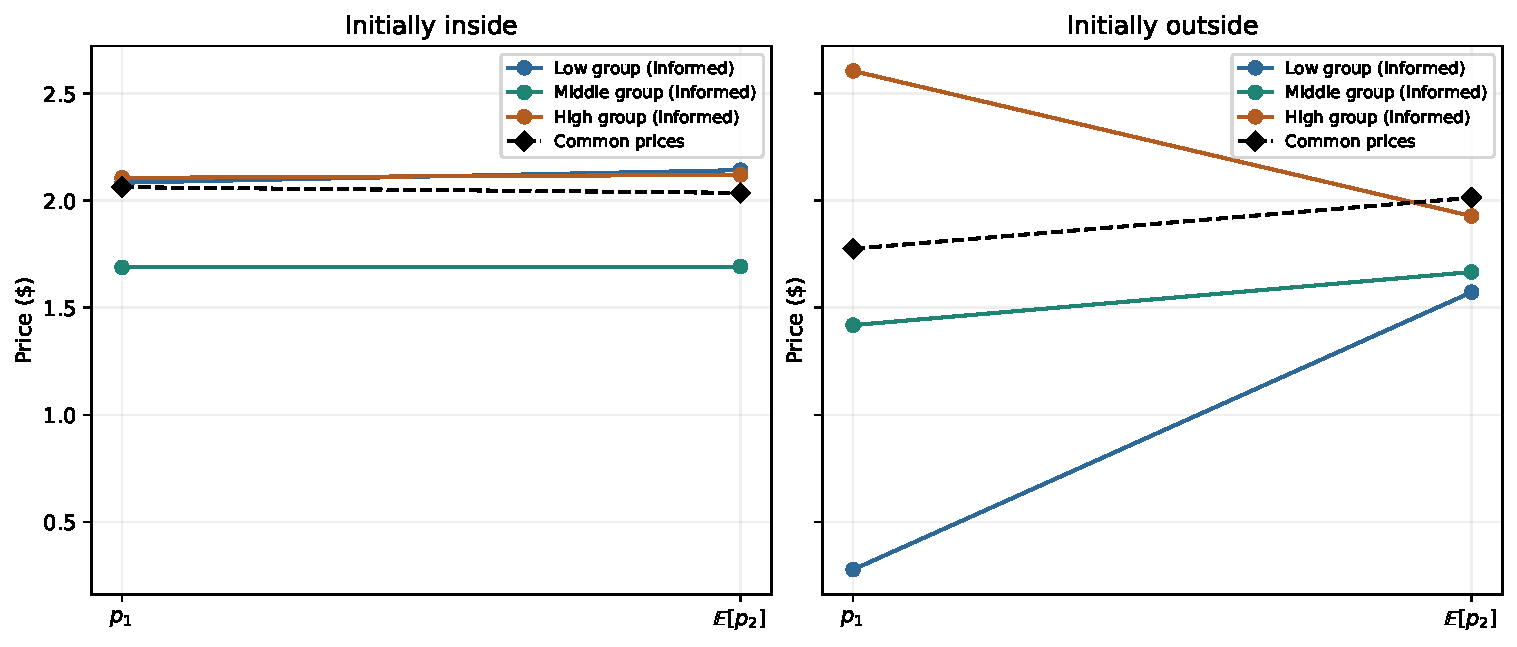
\includegraphics[width=.98\textwidth,height=.68\textheight,keepaspectratio]{assets/quantified_theory/berry/information_price_paths_comparison.pdf}
  \par\smallskip\footnotesize Berry versus not berry. Fitted-distribution baseline;
  solid paths average informed prices within novelty groups.
\end{frame}

\gdef\shortbuttons{\hyperlink{short-revised-paths}{\beamergotobutton{Back to Plain Price Paths}}}
\begin{frame}[label=short-other-paths,noframenumbering]{Other Flavor: Informed and Common Price Paths}
  \centering
  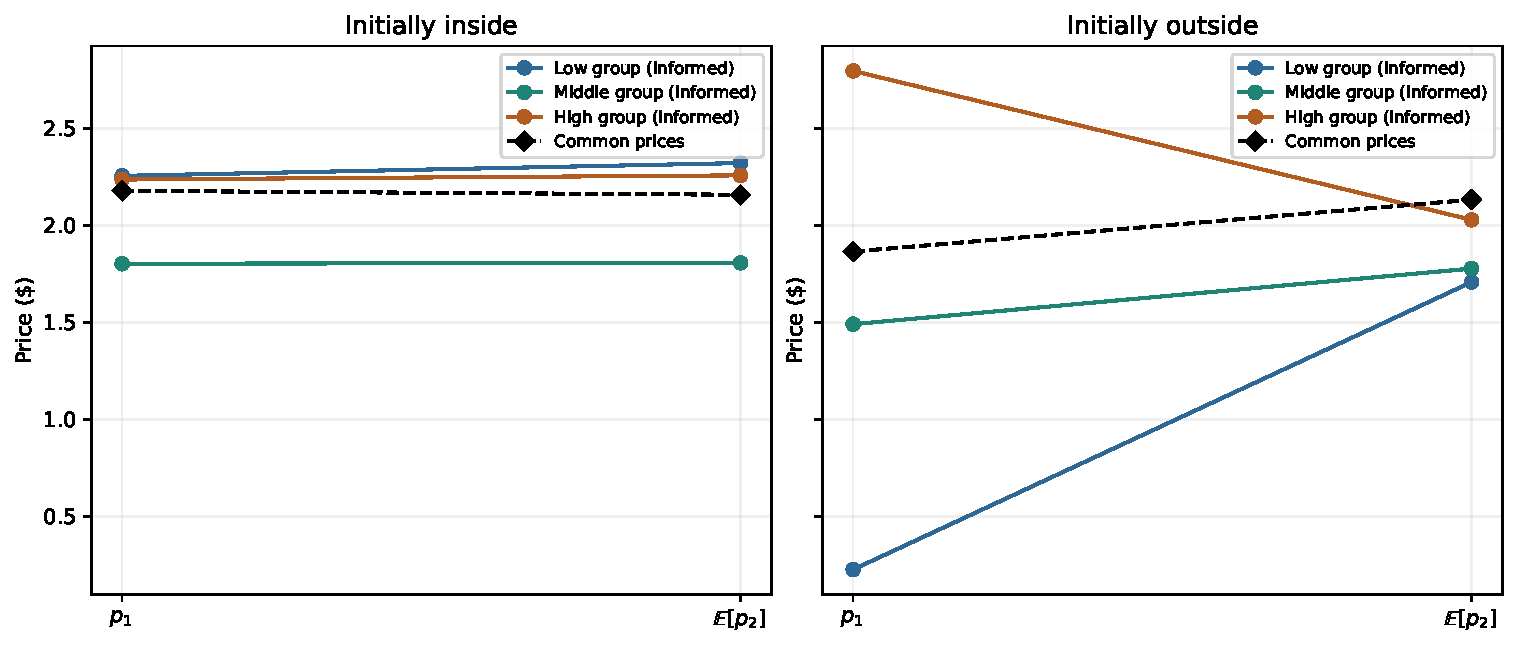
\includegraphics[width=.98\textwidth,height=.68\textheight,keepaspectratio]{assets/quantified_theory/other/information_price_paths_comparison.pdf}
  \par\smallskip\footnotesize Other versus plain, berry or nonpurchase.
  Fitted-distribution baseline; ``other'' is the residual flavor category.
\end{frame}

\gdef\shortbuttons{\hyperlink{short-revised-revenue}{\beamergotobutton{Back to Plain Revenues}}}
\begin{frame}[label=short-all-flavors,noframenumbering]{Informed versus Common Revenue: All Three Flavors}
  \centering\small
  \begin{tabular}{llrrr}\toprule
Focal flavor & Initial history & Informed & Common & Gain\\\midrule
Plain & Inside & 1.6639 & 1.6059 & 0.0581 \\
Plain & Outside & 1.0993 & 0.9774 & 0.1219 \\
Berry & Inside & 1.3968 & 1.3511 & 0.0456 \\
Berry & Outside & 0.8991 & 0.8106 & 0.0886 \\
Other & Inside & 1.6583 & 1.6005 & 0.0578 \\
Other & Outside & 1.0950 & 0.9739 & 0.1212 \\
\bottomrule\end{tabular}

  \par\medskip\footnotesize Fitted-distribution baseline. Dollars per model consumer over two periods.
  Inside/outside is relative to each focal flavor; the two policies use the same persistent types.
\end{frame}

\gdef\shortbuttons{\hyperlink{short-50}{\beamergotobutton{Back to Conclusion}}}
\begin{frame}[label=short-51,noframenumbering]{Next Steps}
  \begin{itemize}
    \item Add firm learning to supply side.
    \item Extend market structure on supply.
    \item Add more product attributes to empirical estimation.
    \item Estimate unobserved quality in BLP fashion.
  \end{itemize}
\end{frame}


% Details moved from the main deck
\gdef\shortbuttons{\hyperlink{short-29}{\beamergotobutton{Back}}}
\begin{frame}[label=short-likelihood,noframenumbering]{Simulated Household Likelihood}
  \footnotesize
  Standard normal draws generate persistent household coefficients:
  \[
    \nu_i=(\nu_{\gamma i},\nu_{\phi i},\nu_{\alpha i})\sim\mathcal N(0,I_3),
    \qquad
    \begin{aligned}
      \gamma_i&=\mu_\gamma+\sigma_\gamma\nu_{\gamma i},\\
      \phi_i&=\mu_\phi+\sigma_\phi\nu_{\phi i},\\
      \alpha_i&=-\exp(\mu_{\log a}+\sigma_{\log a}\nu_{\alpha i}).
    \end{aligned}
  \]
  \vspace{-1ex}
  \begin{tcolorbox}[boxsep=1pt,top=1pt,bottom=1pt]
    \vspace{-2ex}
    \begin{align*}
      L_i(\theta)
        &=\int\!\left[\prod\nolimits_{t=1}^{T_i}P(y_{it}\mid\nu,\theta)\right]
             f_{\mathcal N}(\nu)\,d\nu,\\
      \widehat L_i(\theta)
        &=\frac{1}{R}\sum\nolimits_{r=1}^{R}\prod\nolimits_{t=1}^{T_i}
             P(y_{it}\mid\nu_{ir},\theta),\qquad R=128,\\
      \widehat\theta&=\arg\min\nolimits_\theta\left[-\sum\nolimits_{i=1}^{N}\log\widehat L_i(\theta)\right].
    \end{align*}
    \vspace{-2ex}
  \end{tcolorbox}
  \vspace{-1ex}
  \begin{itemize}
    \item $\theta$: estimated means, standard deviations, and common utility coefficients.
    \item $f_{\mathcal N}$: standard normal density. Each draw gives one household type,
      held fixed across weeks; average over types after multiplying over weeks.
  \end{itemize}
\end{frame}

\gdef\shortbuttons{\hyperlink{short-34}{\beamergotobutton{Back}}}
\begin{frame}[label=short-40,noframenumbering]{Information Comparison with Restricted Learning}
  \begin{itemize}
    \item Informed: the firm observes the consumer's $\gamma$.
    \item Common: the firm knows the distribution of $\gamma$ and offers one price across types.
    \item Both observe purchase history and adapt the second price to plain versus not plain.
    \item Common-price beliefs remain fixed, as in the theory; consumer types persist.
  \end{itemize}
  \begin{tcolorbox}
    Evaluate both policies on the same consumers over two periods.
  \end{tcolorbox}
\end{frame}

\gdef\shortbuttons{\hyperlink{short-34}{\beamergotobutton{Back}}}
\begin{frame}[label=short-revised-revenue,noframenumbering]{Revenue under the Same Persistent Novelty Types}
  \centering
  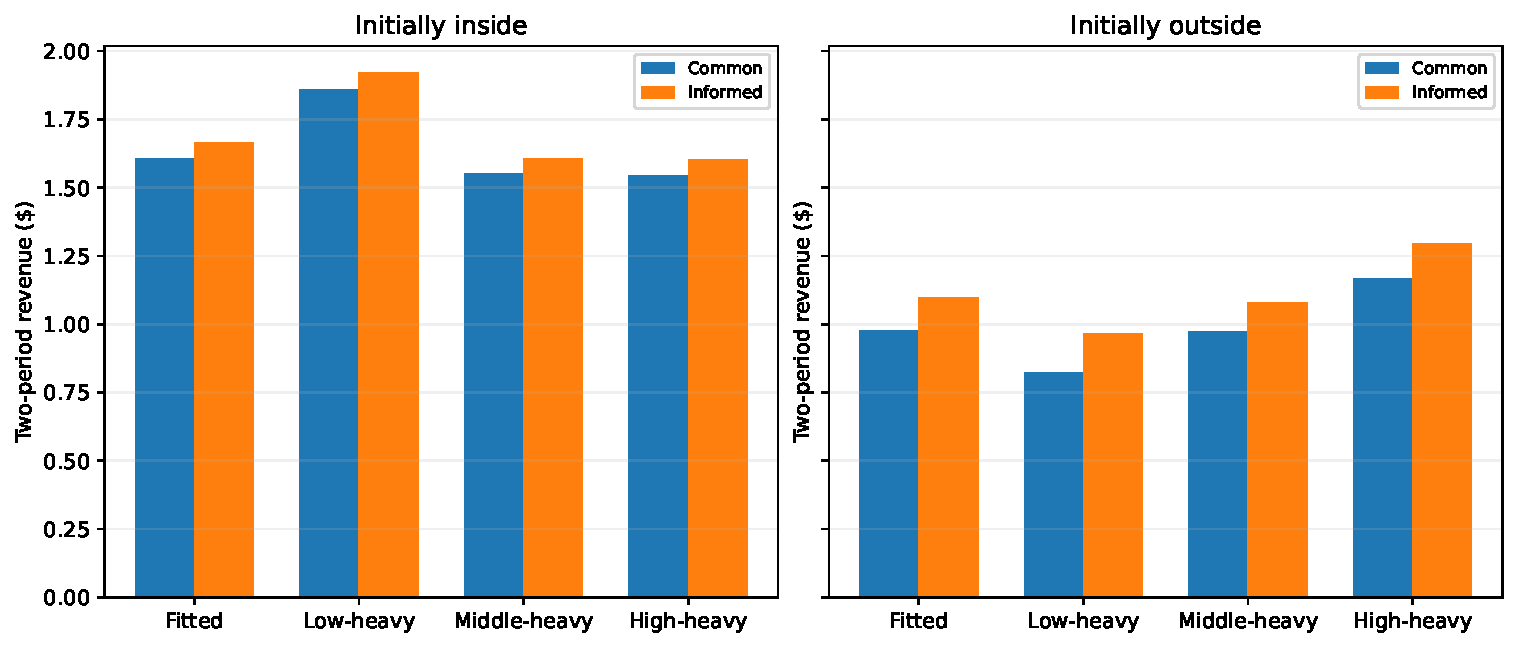
\includegraphics[width=.98\textwidth,height=.68\textheight,keepaspectratio]{assets/quantified_theory/plain/information_revenues.pdf}
  \par\smallskip\footnotesize Expected two-period revenue per model consumer; zero marginal cost.
  Common prices are history-adaptive, with novelty hidden and fixed beliefs.
\end{frame}

\gdef\shortbuttons{\hyperlink{short-34}{\beamergotobutton{Back}}}
\begin{frame}[label=short-revised-table,noframenumbering]{Revenue Comparison by Initial History and Prior}
  \centering\small
  \begin{adjustbox}{max width=\linewidth}
    \begin{tabular}{llrrr}\toprule
Initial state & Distribution & Informed & Common & Gain\\\midrule
$j$ & Fitted distribution & 1.6639 & 1.6059 & 0.0581 \\
$0$ & Fitted distribution & 1.0993 & 0.9774 & 0.1219 \\
$j$ & Low more likely & 1.9227 & 1.8603 & 0.0624 \\
$0$ & Low more likely & 0.9671 & 0.8231 & 0.1440 \\
$j$ & Middle more likely & 1.6051 & 1.5510 & 0.0542 \\
$0$ & Middle more likely & 1.0803 & 0.9736 & 0.1067 \\
$j$ & High more likely & 1.6015 & 1.5435 & 0.0580 \\
$0$ & High more likely & 1.2952 & 1.1669 & 0.1283 \\
\bottomrule\end{tabular}

  \end{adjustbox}
  \par\smallskip\footnotesize Dollars per model consumer over two periods.
  Both regimes adapt second prices to history; only novelty information differs.
\end{frame}
